% ---------------------------  Introdução ------------------------------- %
\chapter{Introdução}

O Plano Nacional de Educação estabelece a seguinte meta: "Oferecer educação em tempo integral em, no mínimo, 50\% das escolas públicas, atendendo, pelo menos, 25\% dos alunos da educação básica." Essa meta reflete a visão da escola não apenas como um local de aprendizado acadêmico, mas como uma instituição que molda cidadãos para o mundo.

 Os dados do Instituto Nacional de Estudos e Pesquisas Educacionais Anísio Teixeira (INEP) indicam um aumento no acesso à educação entre jovens e adolescentes. Se olharmos para os dados de aprovação é perceptível uma melhora ao longo dos anos da série, sendo ela cerca de 76\% em 2007 e 86\% em 2022 para alunos do ensino médio.

Quando olhando para o desempenho dos estudantes do Brasil o cenário não é favorável. De acordo com o Program for International Student Assessment (PISA), que compara o desempenho de estudantes em nível internacional, os alunos brasileiros estão aquém da média dos estudantes de países participantes da OCDE desde o início da aplicação dos testes no ano de 2000. A nível nacional, o Índice de Desenvolvimento da Educação Básica (IDEB) aponta que o desempenho médio no ensino fundamental está abaixo do necessário para se equiparar aos países com alta qualidade educacional. Ademais, quando olhamos para as notas obtidas no Exame Nacional do Ensino Médio (ENEM) vemos notas baixas em relação à escala de notas possíveis.

\begin{figure}[H]
    \centering
    \caption{Evolução de notas do ENEM}
    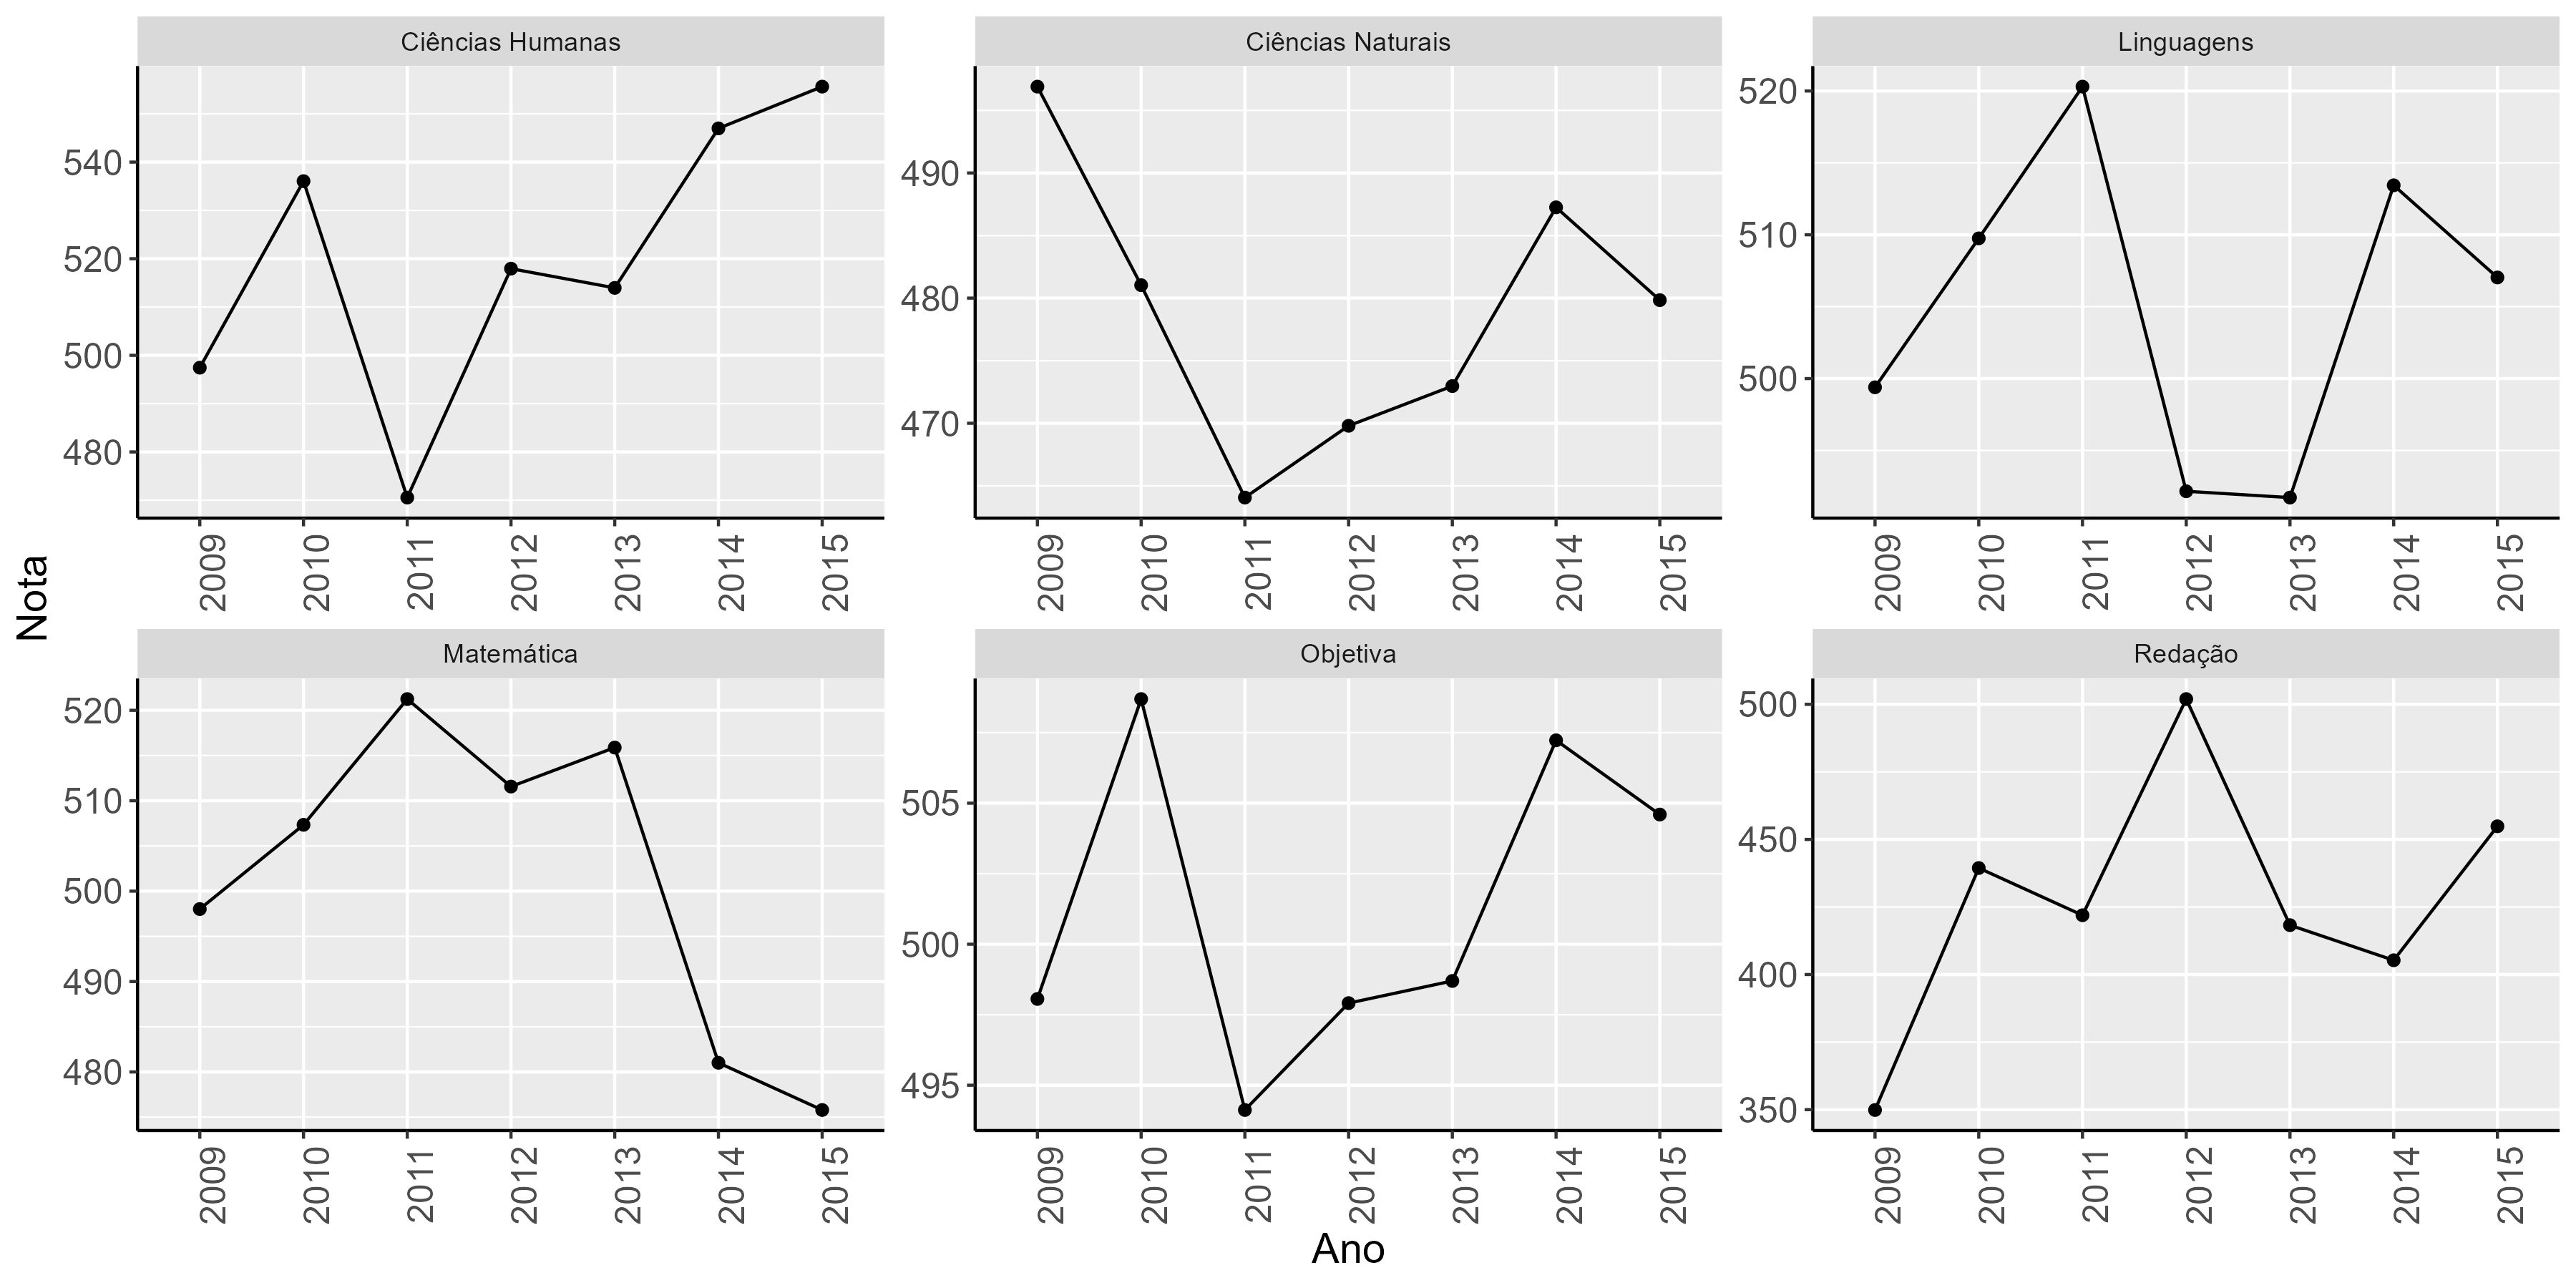
\includegraphics[width=0.95\textwidth]{Charts/serie_media_notas.png}
    \legend{Fonte: Elaboração própria com dados do INEP.}  
    \label{fig:serie_medi_notas}
\end{figure}

De acordo com a Pesquisa Nacional por Amostra de Domicílios Contínua (PNAD), em 2022, apenas um pouco mais da metade da população brasileira completou o ensino básico, enquanto 18\% dos jovens de 14 a 29 anos (cerca de 52 milhões de pessoas) não concluíram o ensino médio, seja por falta de frequência ou abandono. 

\begin{figure}[H]
    \centering
    \caption{Evolução dos indicadores educacionais}
    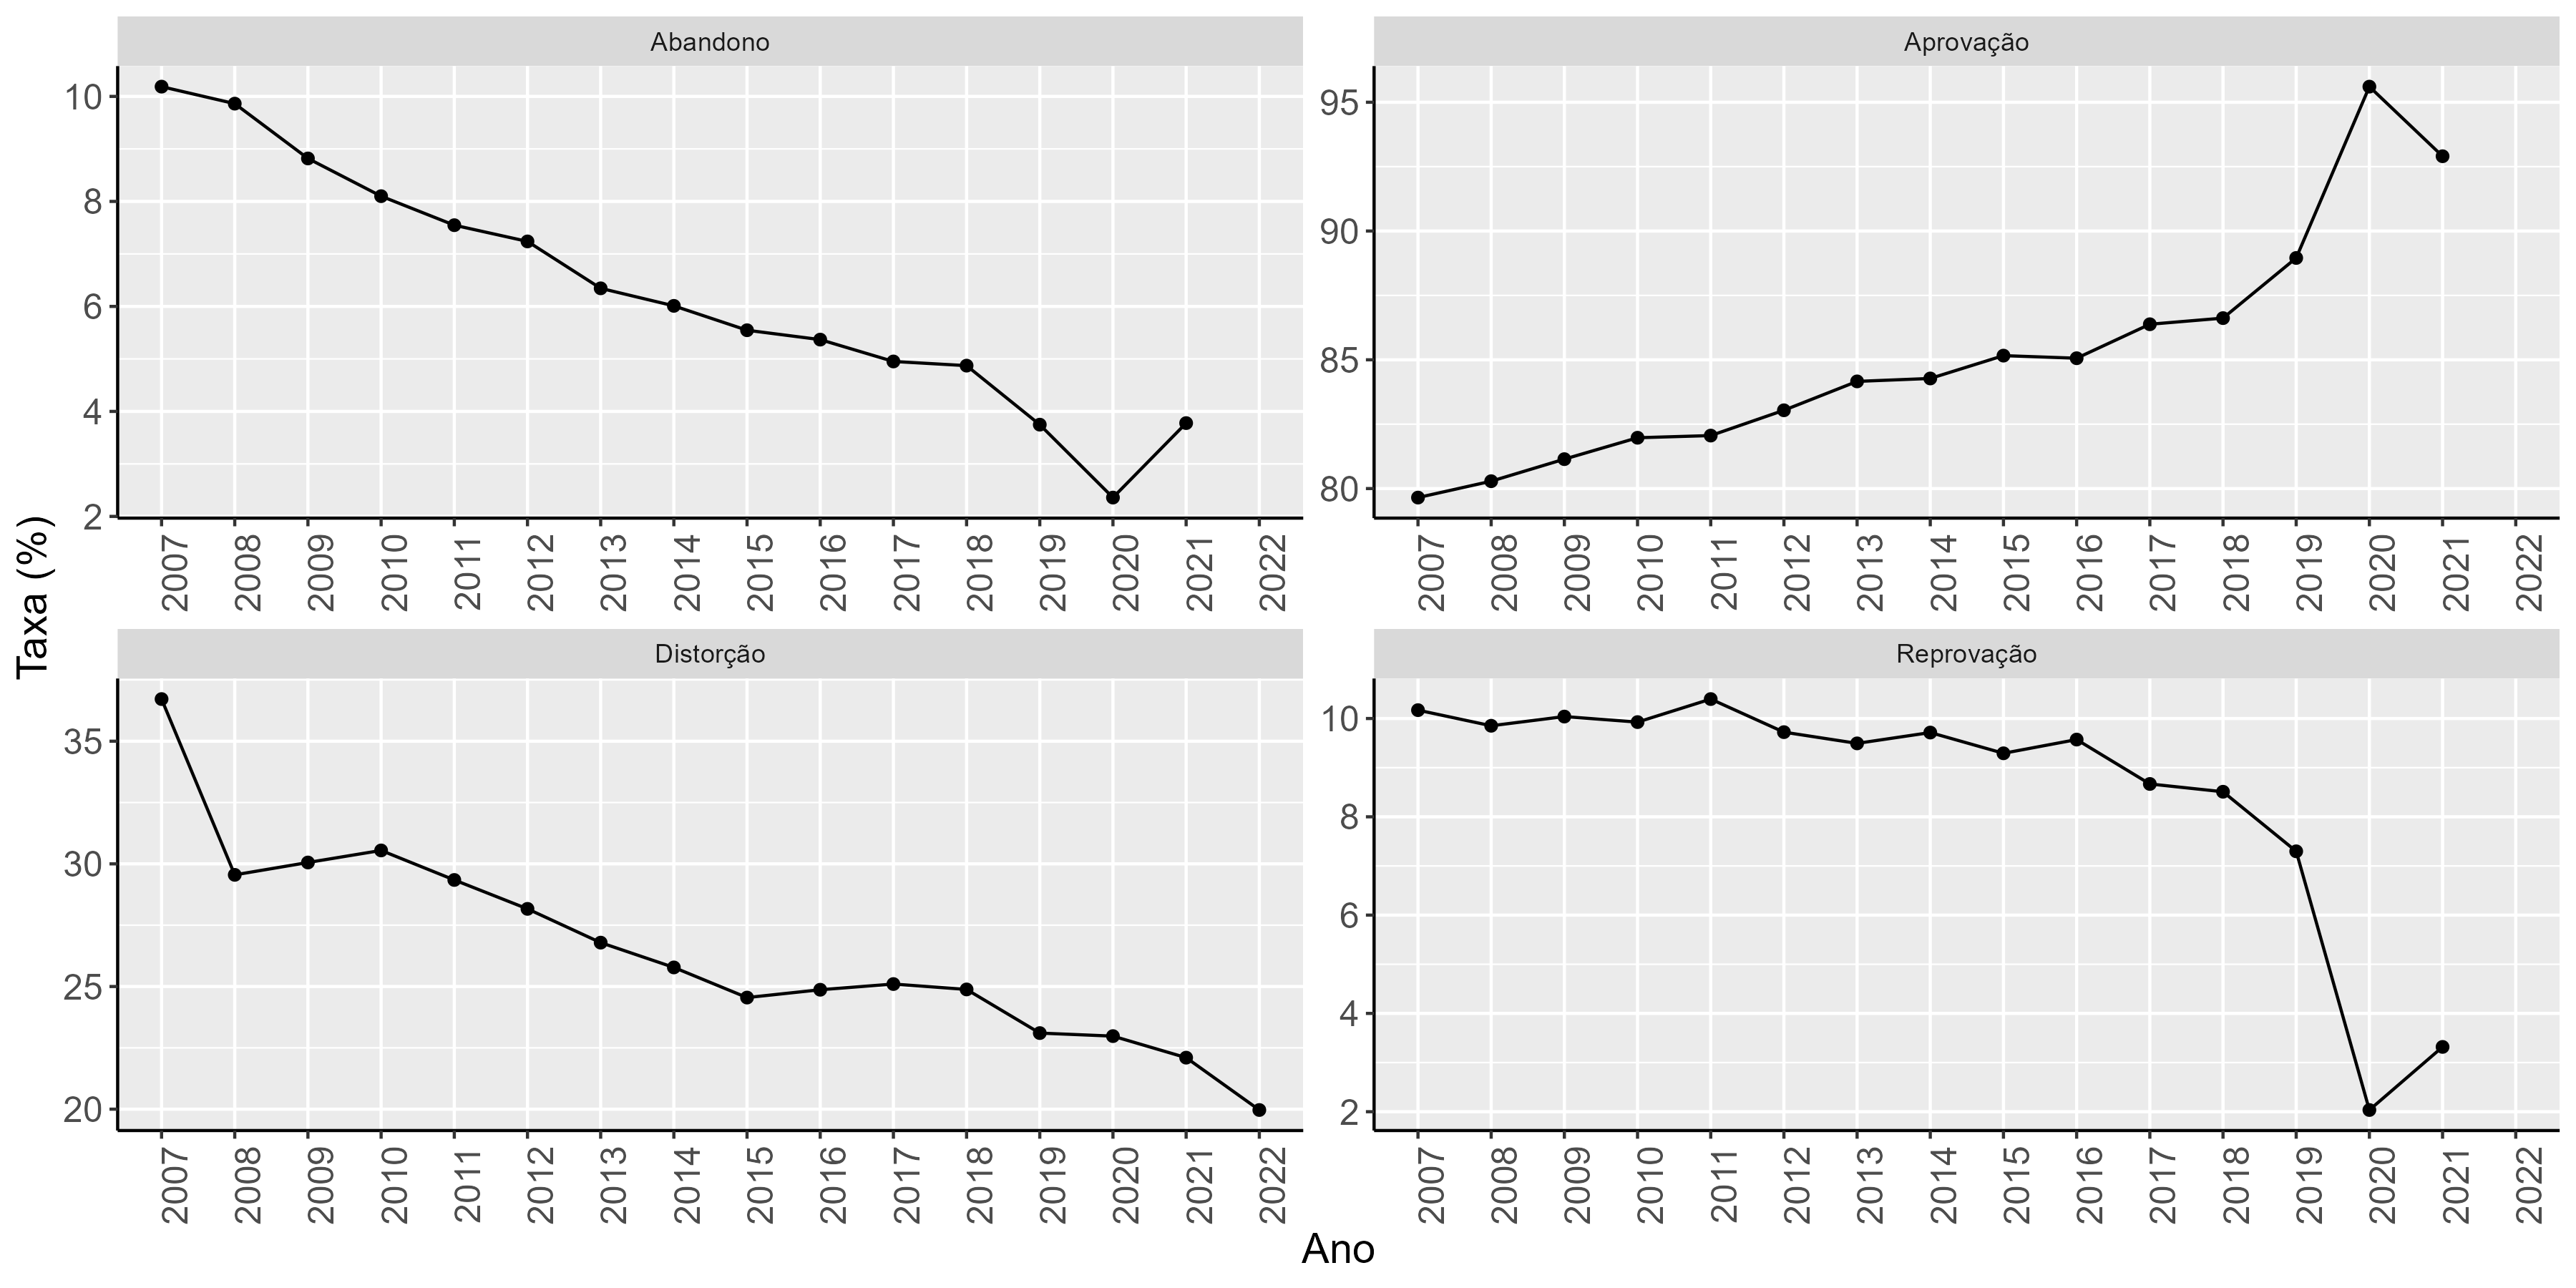
\includegraphics[width=0.95\textwidth]{Charts/serie_media_indicadores.png}
    \legend{Fonte: Elaboração própria com dados do INEP.}  
    \label{fig:serie_medi_indicadores}
\end{figure}

Diante desse cenário, os formuladores de políticas públicas buscam aprimorar continuamente a qualidade da educação. Sendo uma das medidas adotadas a expansão da jornada escolar, alcançada por meio de programas que aumentam a carga horária diária ou o número de dias letivos. Esses programas incluem atividades extracurriculares, reforço escolar, alimentação e orientação de vida, com o objetivo de transformar a escola em um agente integral na formação dos alunos como cidadãos.

No Brasil, essa abordagem é respaldada pelo Plano Nacional de Educação e foi implementado a partir de 2008, começando com o programa "Mais Educação". Este programa do governo federal visava estender a jornada escolar para pelo menos 7 horas diárias, em comparação às 4 horas de uma escola comum.

Para o ensino médio, o programa federal "Ensino Médio Integral" (EMI) foi lançado em 2004 como uma parceria público-privada. O EMI tem como objetivo formar os alunos em aspectos cognitivos, profissionais, pessoais e sociais, além de adotar critérios de gestão que incluem incentivos e critérios de contratação.

Neste trabalho, buscamos compreender se o programa EMI está cumprindo seu propósito de melhorar a qualidade da educação brasileira. Utilizaremos o método de \textit{staggered difference in differences} por \cite{CB_2021}, uma abordagem inédita para avaliar o programa ao nível desejado.

É relevante observar que vários estudos anteriores exploraram o potencial impacto de programas de ensino integral no Brasil, apresentando resultados mistos, como evidenciado por \cite{Oliveira_2008}, \cite{Almeida_2016}, \cite{Pereira_2011}, \cite{Filho_2012}, \cite{Xerxenevsky_2012}, \cite{Oliveira_2018} \cite{Kawahara_2019}. Analisaremos esses resultados de forma mais detalhada no capítulo subsequente.

A estrutura deste trabalho é a seguinte: na seção \ref{revisao}, analisaremos a literatura sobre os efeitos do ensino em tempo integral, tanto no Brasil quanto no cenário global. Na seção \ref{programa}, exploraremos as características, o funcionamento e os objetivos do programa EMI. A seção \ref{dados} apresentará as fontes para os dados que serão utilizados no trabalho. Finalmente, a seção \ref{ecomometria} descreverá o método causal aplicado e na seção \ref{resultados} apresentaremos os resultados obtidos, bem como a comparação deles com a literatura.

Assim, este trabalho visa contribuir para o crescente corpo de literatura sobre os efeitos de programas de ensino em tempo integral em todo o mundo, oferecendo insights que podem auxiliar na avaliação, formulação e implementação de políticas públicas educacionais.

% --------------------------- Desenvolvimento ------------------------ %
\chapter{Revisão de Literatura} \label{revisao}

O tema da ampliação da jornada escolar tem sido objeto de investigação por diversos autores em contextos globais. A seguir, apresentamos uma variedade de estudos que oferecem insights valiosos sobre essa temática diversificada, abordando uma ampla gama de resultados, metodologias e amostras. A heterogeneidade de resultados pode ser atribuída, em grande parte, à multiplicidade de abordagens e características dos programas analisados.

\section{Resultado Teórico} \label{teoria}

Baseando-nos no modelo proposto por \cite{Levin_1987}, supomos que o aluno realiza duas atividades de produção: a atividade escolar \(Q_1\) e outra atividade \(Q_2\). As funções de quantidade são expressas como funções positivas na seguinte forma funcional:

\begin{equation}
\begin{aligned}
& Q_1 = f(C, S) \cdot e_1^{\alpha_1} + t_1^{\beta_1} \\
& Q_2 = k(X) \cdot e_2^{\alpha_2} + t_2^{\beta_2} \\
\end{aligned}
\end{equation}

Aqui, \(e_i\) representa o esforço alocado para a atividade, \(t_i\) o tempo dedicado a ela, \(p_i\) são os preços de cada atividade, \(\alpha_i\) e \(\beta_i\) são parâmetros tecnológicos associados a cada atividade, assumidos como positivos. Além disso, \(C\) representa o nível de capacidade do aluno, \(S\) o nível de recursos de aprendizagem disponíveis e \(X\) são outros fatores externos à escola.

Portanto, o estudante resolverá o seguinte problema de otimização:

\begin{equation}
\begin{aligned}
\max \quad & U = p_1 \cdot F(Q_1) + p_2 \cdot G(Q_2) \\
\textrm{s.a.} \quad & t_1 + t_2 \leq T\\
& e_1 \cdot t_1 + e_2 \cdot t_2 \leq E
\end{aligned}
\end{equation}

Ao maximizar, obtém-se o seguinte resultado de equilíbrio:

\begin{equation}
    \frac{p_1 \cdot (\partial F/ \partial Q_1)Q_1^*}{p_2 \cdot (\partial G/ \partial Q_2)Q_2^*} = \frac{k(X) \alpha_2}{f(C,S)\alpha_1} \cdot \frac{e_1^{*1-\alpha_1}t_1^{*1-\beta_1}}{e_2^{*1-\alpha_2}t_2^{*1-\beta_2}}
\end{equation}

Ao analisar o equilíbrio do modelo proposto, conclui-se que não existem cenários em que haja ganhos significativos na produção do aluno caso haja somente aumento no tempo dedicado à atividade. Isso decorre da observação de reduções no esforço quando o tempo de estudo é aumentado, resultando em resultados nulos ou até mesmo negativos.

No entanto, sob as características do programa, o equilíbrio pode ser interpretado de forma mais abrangente. Como detalhado no capítulo \ref{programa}, o EMI não apenas aumenta a carga horária, mas também introduz dispositivos que renovam o ambiente escolar, como recursos de aprendizagem e aprimoramento da gestão. Portanto, em termos do modelo teórico, podemos interpretar o programa como uma mudança nos coeficientes de produtividade da função de produção (\(\alpha_i\), \(\beta_i\)).

Consequentemente, podemos concluir que o programa resulta em um aumento na produtividade dos alunos, permitindo que eles aloquem mais tempo e esforço na atividade escolar conforme a produtividade de aprendizagem aumenta em relação à produtividade de outras atividades, conforme indicado pelos autores.

Com base nas conclusões teóricas estabelecidas, buscaremos testar se a implementação do programa EMI tem um impacto positivo nos resultados educacionais das escolas brasileiras, conforme desenvolvido no texto acima.
 
\section{Evidências ao redor do mundo}

Em um contexto latino americano, \cite{Bellei_2009} busca compreender como os estudantes chilenos de ensino médio foram afetados pelo programa de extensão da jornada escolar. Utilizando a metodologia de diferenças em diferenças, o autor encontra efeitos positivos em testes de matemática e português.

Segundo \cite{Meroni_2016}, a extensão da jornada escolar pode influenciar positivamente o desempenho acadêmico, parte de um processo cumulativo. Os autores propuseram uma análise abrangente dessas dinâmicas, examinando estudantes italianos de ensino médio no período de 2007 a 2010. Utilizando dados do Ministério de Educação, aplicaram o método de diferenças em diferenças com base na segunda fase do programa Quality and Merit Project (PQM). Os resultados da pesquisa indicam que, para os estudantes do sexo masculino, uma maior exposição à matemática está associada a um aumento na aversão a essa disciplina e a uma maior ansiedade diante de avaliações de linguagem. Por outro lado, para as estudantes do sexo feminino, a exposição à matemática parece contribuir para a redução da aversão a essa matéria e para um melhor desempenho em disciplinas de linguagem.

\section{Evidências para o Brasil}

No contexto brasileiro, encontramos uma série de estudos que examinam os efeitos da carga horária escolar no desempenho dos alunos. Um estudo notável conduzido por \cite{Filho_2012} utilizou dados do Sistema de Avaliação da Educação Básica (SAEB) de 2003 para investigar os determinantes do desempenho de alunos de escolas públicas no Brasil. Este estudo revelou que alunos que frequentavam a escola por mais de 4 horas diárias apresentavam maior proficiência em matemática em comparação àqueles com menos de 4 horas de aulas diárias.

Outra pesquisa relevante, realizada por \cite{Oliveira_2008}, utilizou dados do SAEB referentes a 2005, com foco nos alunos da 4ª série do ensino fundamental. Neste estudo, foram aplicadas técnicas de \textit{matching} para investigar se a redução do tamanho das turmas e o aumento da carga horária escolar influenciaram o rendimento dos alunos. Os resultados apontaram uma estimativa de tratamento médio de 8,36 pontos na proficiência em matemática para os alunos que experimentaram um acréscimo de uma hora na jornada diária, indicando uma relação positiva entre a carga horária e o desempenho acadêmico.

Por outro lado, uma pesquisa conduzida por \cite{Aquino_2011} buscou analisar os efeitos do programa Escola de Tempo Integral. Utilizando dados do Sistema de Avaliação de Rendimento Escolar do Estado de São Paulo (SARESP) dos anos de 2007 e 2008, esta investigação focalizou os alunos da 8ª série do ensino fundamental. Por meio de métodos de \textit{matching} e o método de diferenças em diferenças, a autora não encontrou evidências de efeitos significativos no rendimento em matemática, mas observou efeitos positivos no rendimento em português.

No Brasil, um programa amplamente avaliado é o programa federal Mais Educação. \cite{Pereira_2011} utilizou dados disponibilizados pela secretaria do programa para compreender seus impactos sobre a taxa de abandono escolar, aprovação e rendimento escolar de alunos em todo o país e, especificamente, no estado de Minas Gerais. Por meio do método de diferenças em diferenças, o autor concluiu que o programa não teve efeitos significativos sobre a taxa de aprovação, mas exerceu um efeito positivo na redução da taxa de abandono escolar. Quanto ao rendimento, concluiu que o programa não produziu efeitos significativos sobre os alunos de Minas Gerais.

Utilizando dados da Prova Brasil para os anos de 2007 e 2009 no estado do Rio Grande do Sul, \cite{Xerxenevsky_2012} empregou métodos de propensity score matching e diferenças em diferenças para avaliar o impacto do programa Mais Educação. O autor descobriu que o programa teve impacto positivo no desempenho escolar em língua portuguesa para alunos da 4ª série, mas impacto negativo no desempenho em matemática. Para alunos da 8ª série, não foram observados efeitos significativos para testes de língua portuguesa e matemática.

\cite{Almeida_2016} e \cite{Gandra_2017} utilizaram dados do Censo Escolar em diferentes períodos e aplicaram métodos como propensity score matching e regressão de diferenças em diferenças para avaliar o impacto do programa. Enquanto \cite{Almeida_2016} observou impactos negativos no rendimento em matemática, mas ausência de impacto nas taxas de abandono e aprovação, \cite{Gandra_2017} encontrou impactos negativos no rendimento em matemática e português para as turmas do 5º ano, com maior magnitude nas escolas que aderiram ao programa por mais tempo.

\cite{Oliveira_2018} também utilizou dados do Censo Escolar, aplicando métodos de propensity score matching e regressão com descontinuidade, mas não encontrou melhorias nas taxas de abandono, aprovação, reprovação, proficiências e no Índice de Desenvolvimento da Educação Básica (IDEB).

Há também estudos que buscam compreender outro programa presente no Brasil, o Ensino Médio Integral (EMI), o qual é objeto de estudo do presente texto. Ao estudarem a mesma intervenção utilizando métodos diferentes, \cite{Kawahara_2019} e \cite{Rosa_2022a} chegam a conclusões semelhantes sobre os efeitos do programa nas notas em testes padronizados. O primeiro procura compreender como o programa impacta o rendimento dos alunos de escolas públicas. Utilizando o método de diferenças em diferenças dinâmico, o autor constatou que há efeitos positivos e crescentes no tempo sobre os testes padronizados de matemática e português. O autor também indica a possibilidade de que o programa também traga efeitos indiretos. Esses efeitos podem incluir mudanças resultantes da mobilidade de alunos entre escolas, alterações na estrutura escolar e no ambiente socioeconômico dos alunos, bem como efeitos relacionados à autoseleção de alunos e professores. Já o segundo estuda o mesmo programa, com foco nas escolas de Pernambuco, estado onde o programa se iniciou. Para o contexto deste trabalho, os resultados obtidos por meio do método de \textit{staggered difference in differences} proposto por \cite{CB_2021} mostram que ao longo dos anos após a implementação da política, há um efeito positivo e crescente sobre os resultados dos alunos em testes padronizados, de modo que características observáveis dos alunos possivelmente não alteram os resultados encontrados. 

\section{Evidências de médio e longo prazo}

Outros estudos buscam compreender efeitos além da sala de aula. Para isso, os estudos buscam entender efeitos de médio e longo prazo dos estudantes expostos a programas de ensino integral. Como objeto de estudo, os artigos relacionam o programa com resultados econômicos.

Conforme evidenciado por \cite{Barros_2022}, o ensino médio em tempo integral pode acarretar efeitos positivos a médio e longo prazo tanto para os alunos quanto para a sociedade em geral. Com base nos resultados apresentados pelos autores, espera-se que esses efeitos se manifestem de forma positiva em indicadores como empregabilidade, renda, produtividade e crescimento econômico.

As evidências mostradas por \cite{Dominguez_2020} nos permite observar que ao ser exposto ao programa de ensino médio integral há aumento das chances dos alunos de concluir o ensino básico e superior, sendo este um resultado positivo do programa. Caso a exposição ao ensino médio integral traga efeitos de proficiência, como mostrado por \cite{Barros_2019}, podemos esperar que o aluno possa ter uma elevação em seu rendimento, como evidenciado por \cite{Barros_2021}.
\chapter{O Programa Ensino Médio Integral} \label{programa}
No início dos anos 2000, o Ginásio Pernambucano, o colégio mais antigo do Brasil, passou por uma reforma promovida pela sociedade civil. Uma das mudanças significativas incluiu a transição para o modelo de ensino integral. Desde então, esse programa foi adotado pelo governo federal e expandido para todos os estados do Brasil, com aproximadamente 544 escolas participantes em 2015 \cite{Kawahara_2019}. A expansão do programa é realizada com o apoio de um instituto voltado à políticas educacionais, o Instituto de Corresponsabilidade pela Educação (ICE).

O principal objetivo desse programa é atender à Meta 6 do Plano Nacional de Educação (PNE), que busca expandir o ensino em tempo integral. Para alcançar essa meta, o programa adota uma abordagem pedagógica baseada no conceito de "Projeto de Vida". Isso significa que as escolas não apenas se concentram no desenvolvimento cognitivo dos alunos, mas também no seu desenvolvimento socioemocional. Os estudantes são incentivados a se tornarem protagonistas de suas próprias vidas, tomando decisões responsáveis, enquanto recebem o apoio de profissionais envolvidos ativamente em suas jornadas educacionais.

Além da abordagem pedagógica, o programa também reorganiza a gestão das escolas participantes. Isso envolve critérios específicos para a contratação de professores e gestores, sistemas de incentivos para os educadores e métricas de gestão para avaliar o progresso.

A transição de uma jornada escolar de 4 horas diárias para 9 horas requer modificações na infraestrutura das escolas. Nesse sentido, o instituto colabora com as secretarias de educação na seleção das escolas e, nas fases iniciais do programa, oferece apoio financeiro para a compra de materiais escolares, construção de novas instalações e pagamento de bônus de desempenho e alimentação. Durante essa fase inicial, o instituto também supervisiona de perto a implementação do programa. Uma vez que o programa é estabelecido, as escolas têm mais autonomia para gerenciá-lo, bem como para administrar suas instalações e sistemas, uma vez que o instituto retira sua supervisão direta.

Até o ano de 2022, 6400 das 19870 escolas no Brasil apresentavam o ensino médio integral, estando concentradas nas regiões Sudeste e Nordeste do país, como apresentado na Figura \ref{fig:brazil_schools}. 

\begin{figure}[H]
    \centering
    \caption{Quantidade de escolas com ensino integral no ano de 2022}
    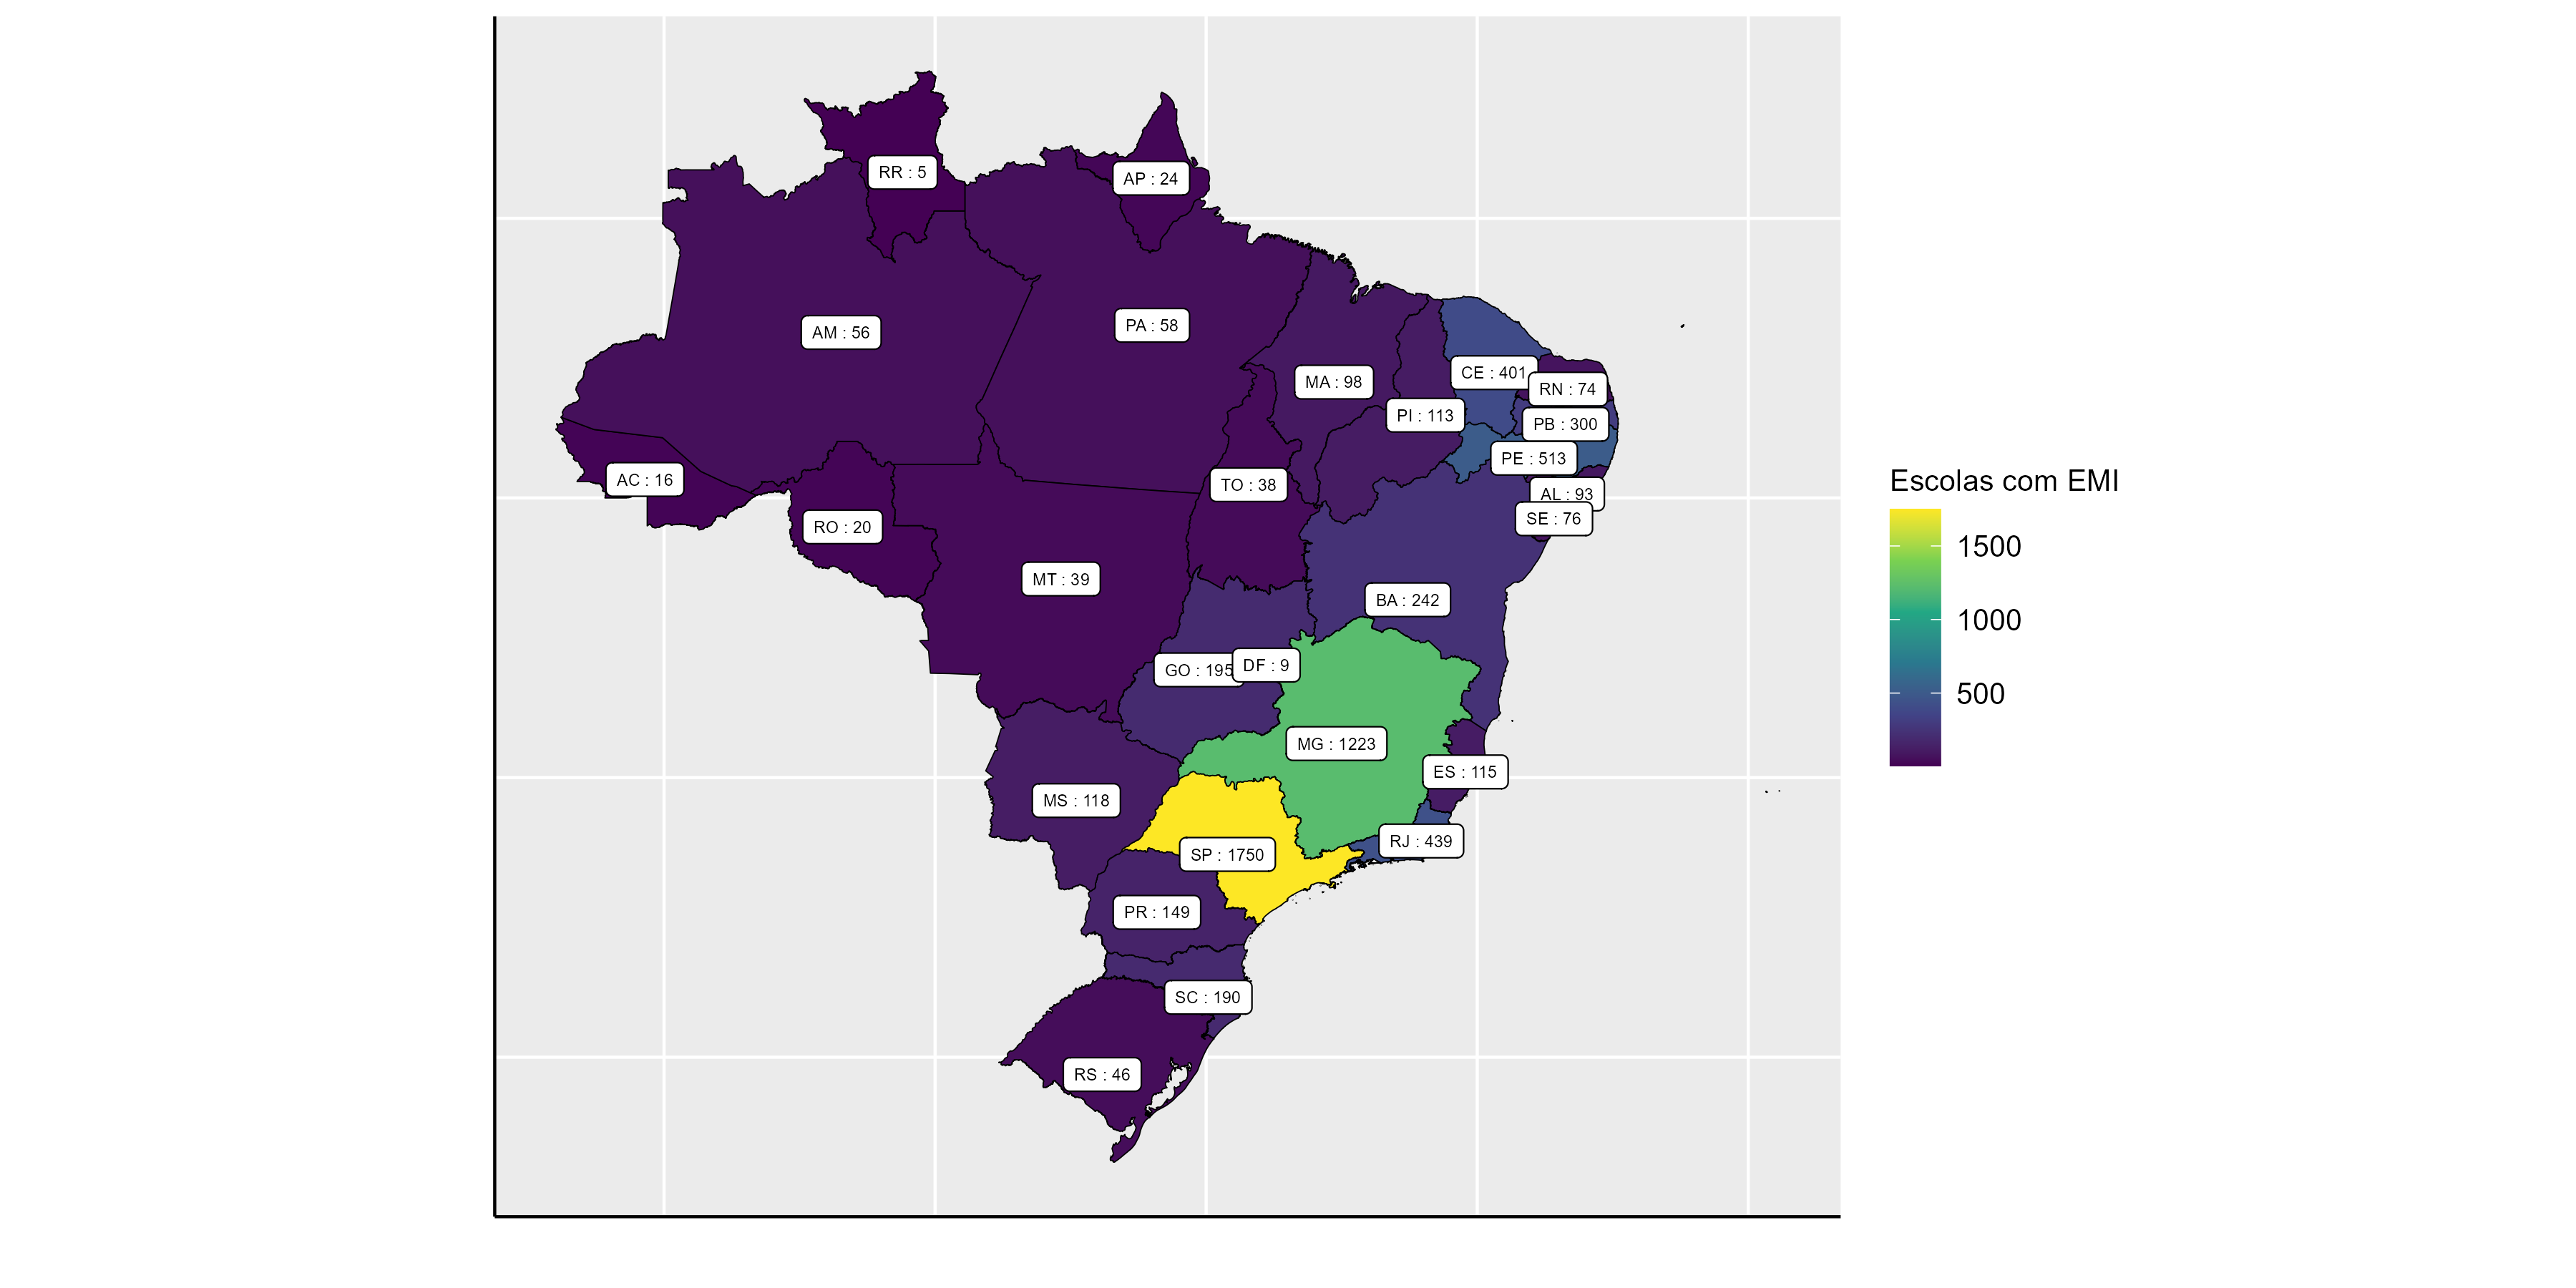
\includegraphics[width=1.15\textwidth]{Charts/brazil_schools.png}
    \legend{Fonte: Elaboração própria com dados do Instituto Sonho Grande, 2024.}  
    \label{fig:brazil_schools}
\end{figure}

\begin{figure}[H]
  \centering
  \caption{Percentual de escolas integrais no ensino médio}
  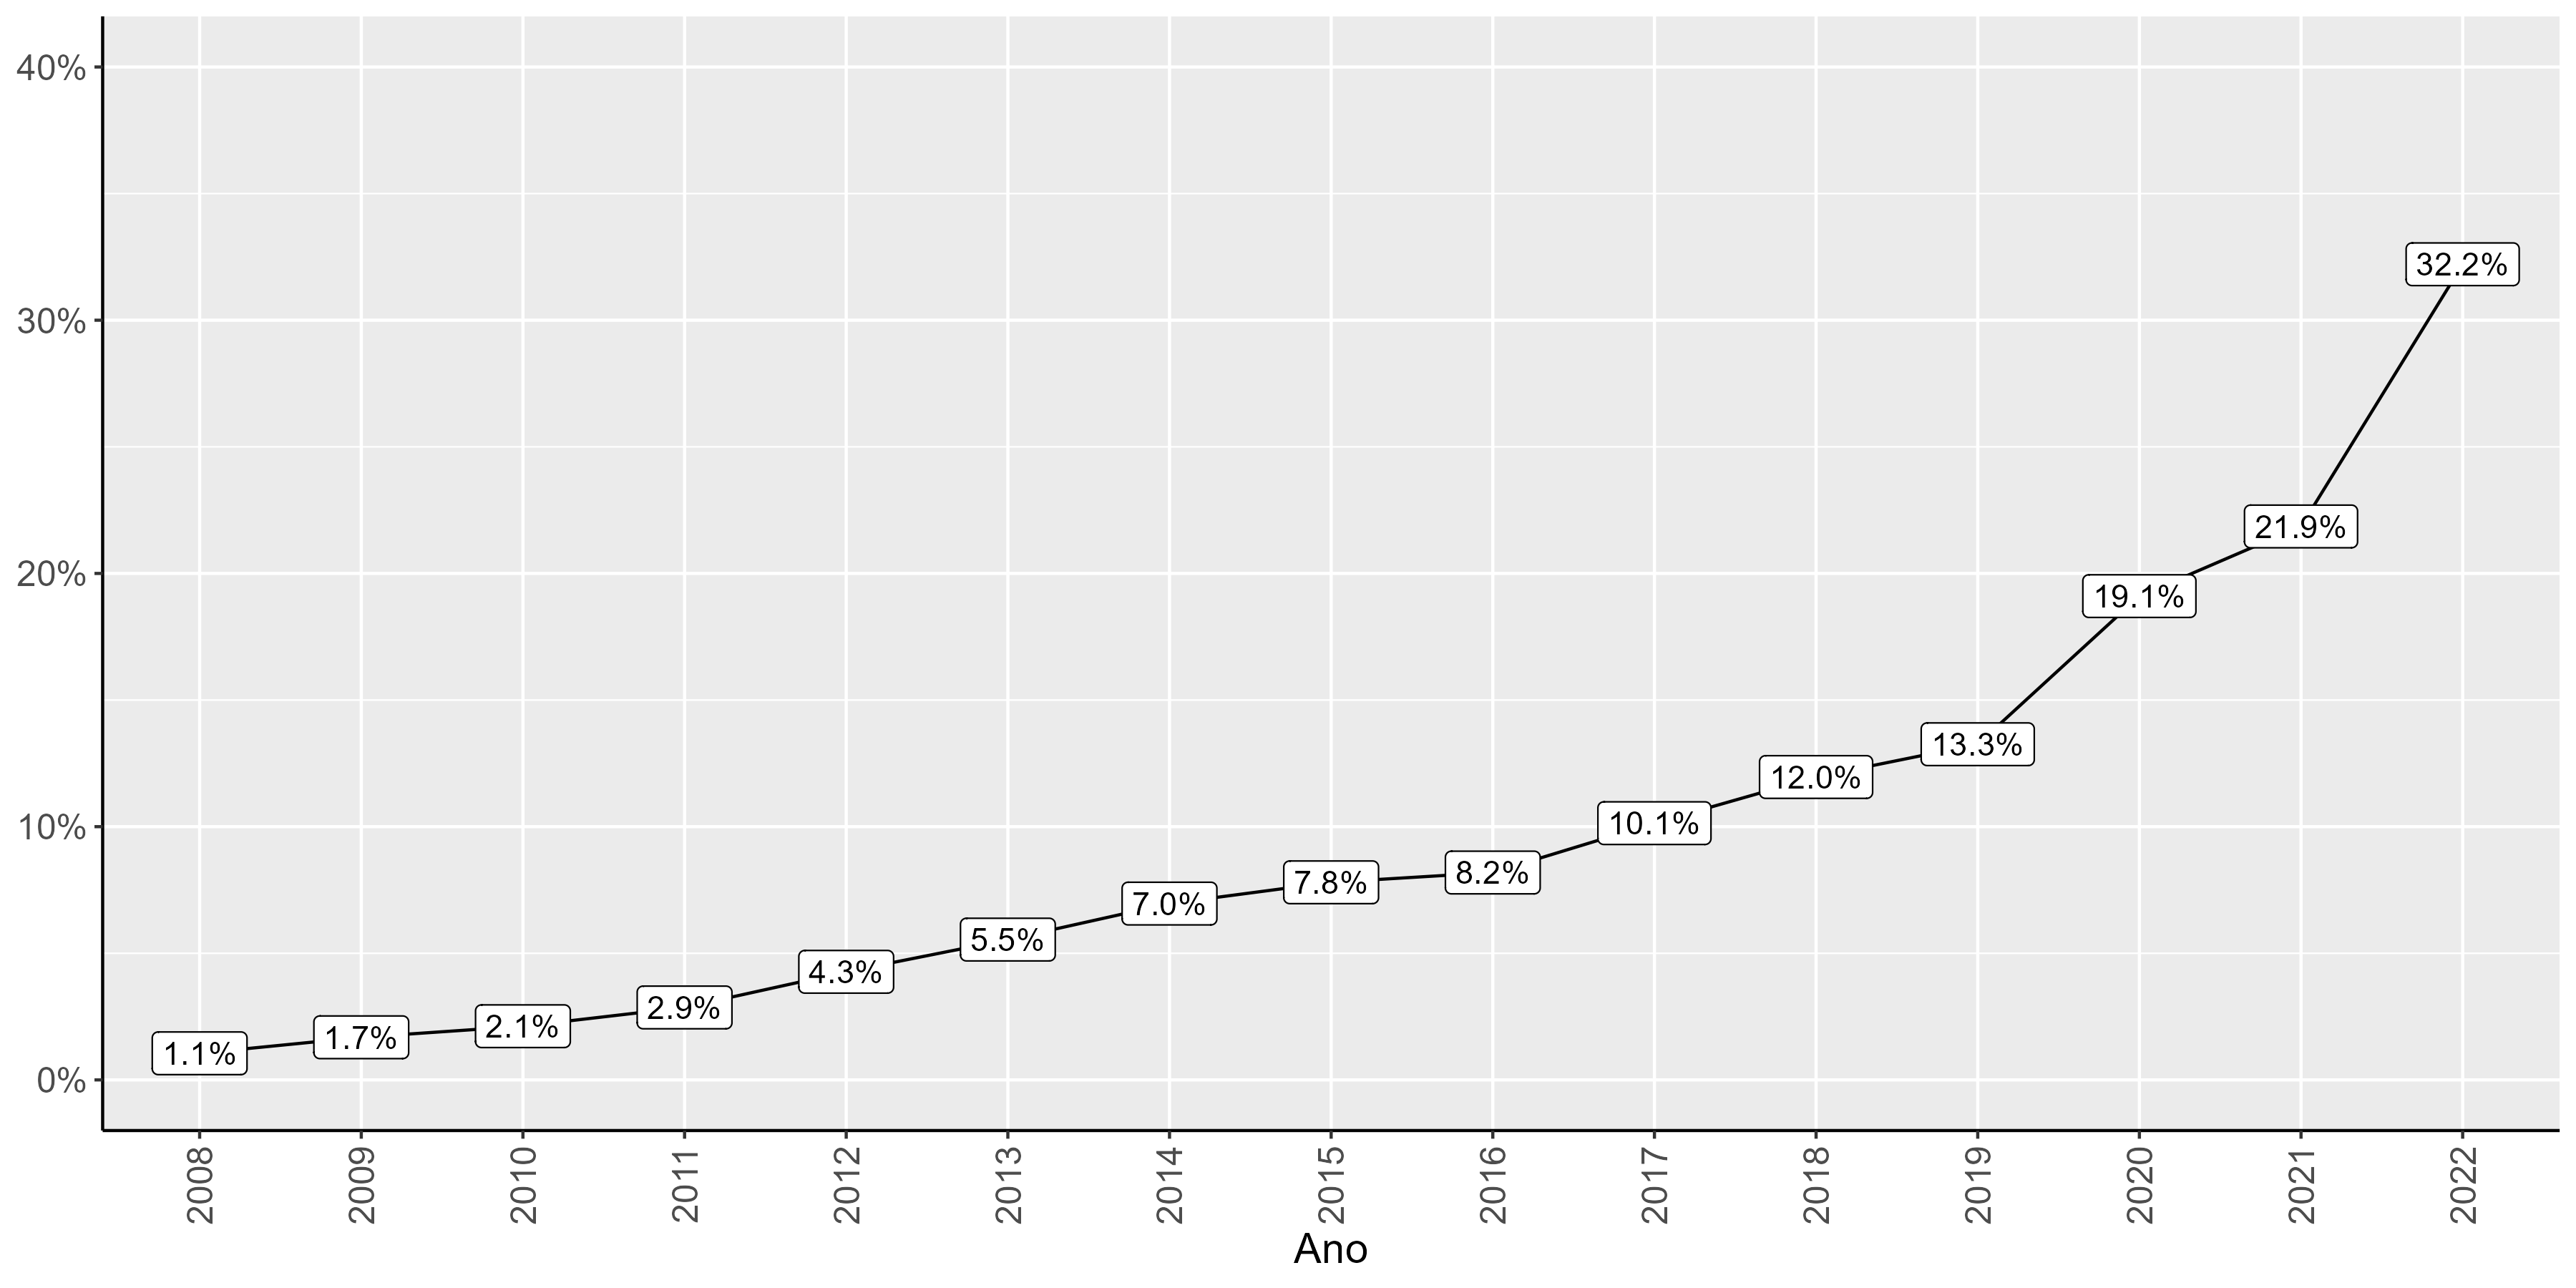
\includegraphics[width=1\textwidth]{Charts/serie_escolas_integral.png}
  \legend{Fonte: Elaboração própria com dados do Instituto Sonho Grande, 2024.}  
  \label{fig:serie_escolas_integral}
\end{figure}
\chapter{Base de Dados} \label{dados}

Os dados utilizados neste trabalho são divididos em dois conjuntos, tendo como fontes o Instituto Nacional de Estudos e Pesquisas Educacionais Anísio Teixeira (INEP), o Instituto Corresponsabilidade pela Educação (ICE) e o Instituto Sonho Grande (ISG).

O Censo Escolar, realizado anualmente pelo INEP, fornece informações detalhadas sobre as estruturas físicas e organizacionais das escolas públicas e privadas do ensino básico no Brasil. Este conjunto de dados oferece um panorama escolar, especialmente para instituições de ensino médio.

Além disso, o Exame Nacional do Ensino Médio (ENEM), também organizado pelo INEP anualmente, é um exame voluntário que avalia o nível de aprendizado dos alunos das escolas públicas e privadas do ensino médio do Brasil em cinco áreas de competência (linguagens, matemática, ciências naturais, ciências humanas e redação). Os resultados do ENEM são frequentemente usados pelos estudantes em suas candidaturas para ingresso no ensino superior, tanto em universidades federais quanto em diversas instituições privadas. Além de avaliar o desempenho dos alunos nessas áreas, o exame inclui um questionário socioeconômico.

Os dados administrativos do ICE apresentam informações sobre as escolas que aderiram ao programa, indicando o ano de ingresso e detalhes dos elementos implementados em cada instituição. 

Os dados do ISG apresentam o ano em que a escola aderiu ao programa, bem como certas características sobre ela.

O primeiro conjunto foi fornecido por \cite{Kawahara_2019}. Ele provêm do INEP e de informações administrativas do ICE. Este conjunto diz respeito aos resultados das escolas nas provas do ENEM  durante os anos de 2009 e 2015, abrangendo escolas de ensino médio situadas nos estados de São Paulo, Rio de Janeiro, Espírito Santo, Ceará, Pernambuco e Goiás. 

Já o segundo conjunto de dados foi construído com base nas informações das escolas que participam do programa, disponibilizadas pelo ISG. Este conjunto diz respeito a indicadores educacionais do INEP (taxa de aprovação, reprovação, abandono e distorção) entre os anos de 2007 e 2022 para escolas localizadas em todo território brasileiro \footnote[1]{\textit{Uma descrição das variáveis presentes em ambos conjuntos está disponível no Apêndice \ref{apendice_descricao}.}}.

Na Tabela \ref{tab:descritiva_resultados} conseguimos ver estatísticas descritivas para as variáveis de resultados acadêmicos, enquanto nas Tabelas \ref{tab:desc_ice} e \ref{tab:desc_censo} é possível observer estatísticas descritivas para as variáveis de caracterísitcas das escolas nos dois conjuntos de dados utilizados. Com base na Tabela \ref{tab:descritiva_resultados} podemos observar o baixo desempenho dos alunos do ensino médio brasileiro no ENEM, sendo seu rendimento médio aquém do nível máximo do teste. No mais, observarmos médias mais baixas em diversos indicadores educacionais entre as escolas tratadas, havendo significância estatística que sustente esta diferença.

\begin{table}[H]
\centering
\caption{Estatísticas descritivas para variáveis de resultados escolares}
\label{tab:descritiva_resultados}
\begin{tabular}{lcccc}
\hline
                          &Média& Desvio Padrão & \multicolumn{2}{c}{Teste-T Para Médias}\\
\cline{4-5}
                          & & & Diferença & P-Valor \\
\hline
Nota em matemática        & 501,4 &74,4 &-32,7& <0,001\\
Nota em linguagens        & 504,8& 49,8&-22,1& <0,001\\
Nota em ciências naturais & 478,8&51,1 &-25,9& <0,001\\
Nota em ciências humanas  & 520,1& 520,1 &-26,2& <0,001\\
Nota em redação           & 427,1& 451,0&-15,1& <0,001\\
Nota geral em objetivas          & 501,4& 51,0&-26,2& <0,001\\
Taxa de abandono          & 6,2&8,7&7,3& <0,001\\
Taxa de reprovação        & 8,5&8,8&5,1& <0,001\\
Taxa de distorção         & 26,3&20,6&21,9& <0,001\\
Taxa de aprovação         & 85,3&13,3&-12,3& <0,001\\ 
\hline
\end{tabular}
    \legend{Fonte: Elaboração própria, 2024.} 
\end{table}

\begin{table}[H]
  \centering
  \caption{Descritivas das características escolares no primeiro conjunto de dados}
  \label{tab:desc_ice}
  \begin{tabular}{lcc}
  & Média& Desvio Padrão \\
  \hline
  Mora com mais de 6 pessoas (\%) & 0.050 & 0.090 \\
  Renda familiar acima de 5 salários mínimos (\%) & 0.170 & 0.251 \\
  Já trabalhou ou procurou emprego (\%) & 0.439 & 0.303 \\
  Número de mulheres no EM 1 & 53.407 & 63.183 \\
  Número de mulheres no EM 2 & 45.012 & 52.181 \\
  Número de mulheres no EM 3 & 40.019 & 46.544 \\
  Zona rural (\%) & 0.038 & 0.192 \\
  Ativa (\%) & 1.000 & 0.000 \\
  Prédio (\%) & 0.990 & 0.101 \\
  Diretoria (\%) & 0.949 & 0.219 \\
  Biblioteca (\%) & 0.558 & 0.497 \\
  Sala de leitura (\%) & 0.478 & 0.500 \\
  Laboratório de informática (\%) & 0.872 & 0.334 \\
  Laboratório de ciências (\%) & 0.453 & 0.498 \\
  Quadra de esportes (\%) & 0.792 & 0.406 \\
  Internet (\%) & 0.967 & 0.178 \\
  Coleta de lixo (\%) & 0.988 & 0.108 \\
  Eletricidade (\%) & 0.999 & 0.030 \\
  Água potável (\%) & 0.958 & 0.201 \\
  Esgoto (\%) & 0.829 & 0.376 \\
  Mulheres no EM 1 (\%) & 0.501 & 0.089 \\
  Mulheres no EM 2 (\%) & 0.528 & 0.095 \\
  Mulheres no EM 3 (\%) & 0.545 & 0.103 \\
  Alunos brancos no EM 1 (\%) & 0.579 & 0.273 \\
  Alunos brancos no EM 2 (\%) & 0.588 & 0.279 \\
  Alunos brancos no EM 3 (\%) & 0.593 & 0.283 \\
  Alunos no EM 1 que utilizam transporte público (\%) & 0.179 & 0.301 \\
  Alunos no EM 2 que utilizam transporte público (\%) & 0.178 & 0.303 \\
  Alunos no EM 3 que utilizam transporte público (\%) & 0.175 & 0.301 \\\hline
  \end{tabular}
      \legend{Fonte: Elaboração própria, 2024.} 
  \end{table}
  
  \begin{table}[H]
    \centering
    \caption{Descritivas das características escolares no segundo conjunto de dados}
    \label{tab:desc_censo}
    \begin{tabular}{lcc}
    & Média& Desvio Padrão \\
    \hline
    Zona rural (\%) & 0.129 & 0.335 \\
    Ativa (\%) & 1.000 & 0.000 \\
    Prédio (\%) & 0.985 & 0.120 \\
    Diretoria (\%) & 0.919 & 0.273 \\
    Biblioteca (\%) & 0.668 & 0.471 \\
    Sala de leitura (\%) & 0.314 & 0.464 \\
    Laboratório de informática (\%) & 0.849 & 0.358 \\
    Laboratório de ciências (\%) & 0.427 & 0.495 \\
    Quadra de esportes (\%) & 0.542 & 0.498 \\
    Internet (\%) & 0.906 & 0.292 \\    
    Coleta de lixo (\%) & 0.924 & 0.266 \\
    Eletricidade (\%) & 0.993 & 0.085 \\
    Água potável (\%) & 0.880 & 0.324 \\
    Esgoto (\%) & 0.600 & 0.490 \\
    \hline
  \end{tabular}
    \legend{Fonte: Elaboração própria, 2024.} 
    \end{table}
\chapter{Estratégia Empírica} \label{ecomometria}

Nesta seção, descreveremos a metodologia que será empregada para avaliar o impacto do Programa Ensino Médio Integral (EMI) no contexto brasileiro. A abordagem metodológica é fundamental para garantir uma análise robusta e precisa dos efeitos do programa. Para isso, utilizaremos o método de \textit{staggered differences in differences} proposto por \cite{CB_2021}.

Como citado na revisão de literatura, diversos trabalhos ao redor do mundo já tentaram adotar estratégias de inferência causal para avaliar programas relacionados ao aumento da carga horária escolar. Para isso, tais estudos tendem a utilizar a metodologia de diferenças-em-diferenças, consolidada na comparação de grupos de tratamento e controle.

Uma das abordagens mais utilizadas é denominada \textit{two-way fixed effect differences in differences}. Em uma especificação estática, podemos escrever tal abordagem da seguinte forma:

\begin{equation}
    Y_{it} = \alpha_0 + \delta D_{i,t} + X_{i,t} + \alpha_i + \alpha_t + \varepsilon_{i,t}
\end{equation}

Supondo que $k$ seja o grupo tratado e $U$ o grupo dos não tratados, podemos escrever a abordagem \textit{two-way fixed effect differences in differences} da seguinte forma:

\begin{equation}
    \hat{\delta}_{kU} = (\overline{Y}_k(1) - \overline{Y}_k(0)) -  (\overline{Y}_U(1) - \overline{Y}_U(0))
\end{equation}

Entretanto, o caráter de certos programas consiste em diferentes grupos de tratamento sendo tratados em diferentes períodos de tempo, ou seja, eles recebem tratamento escalonado. Nesse cenário, vamos supor que o grupo $k$ seja tratado antes do grupo $l$. \cite{Bacon_2021} propõe que o estimador de diferenças em diferenças para este cenário pode ser decomposto da seguinte forma:

\begin{equation}
    \hat{\delta} = \sum_{k \neq U} s_{kU}\hat{\delta}_{kU}+\sum_{k \neq U}\sum_{l>k}s_{kl}[\mu_{kl}\hat{\delta}_{kl} + (1-\mu_{kl})\hat{\delta}_{kl}]
\end{equation}

Como demonstrado por \cite{Bacon_2021}, o estimador pode ser decomposto como uma ponderação dos estimadores de diferenças-em-diferenças entre cada grupo existente na amostra, de modo que a adoção do método em situações de tratamento escalonado pode trazer viés ao estimador através de: i) a descoberta das ponderações faz com que unidades tratadas no meio do painel tenham maior peso no estimador final do que aquelas tratadas no início ou final; e ii) há possibilidade de comparação entre unidades tratadas no começo do painel e unidades tratadas no final do painel, o que pode distorcer o efeito médio do tratamento sobre os tratados (ATT, do inglês \textit{Average Treatment Effect on the Treated}).

Com o objetivo de contornar tais obstáculos, \cite{CB_2021} desenvolveram um estimador para \textit{staggered differences in differences}. Supondo que nenhuma unidade seja tratada no primeiro período de tempo, podemos organizar as unidades de forma que elas participem de um grupo $g \in G$, que indica em qual período o indivíduo foi tratado. Seja $Y_{i,t}$ o resultado potencial do indivíduo $i$ teria no período $t$ caso tenha sido tratado no período $g$. Tendo por base a suposição de amostra aleatória, buscamos o seguinte ATT:

\begin{equation}
    ATT(g,t) = \mathbb{E}[Y_t(g) - Y_t(0)|G_g = 1]
\end{equation}

Para obtermos a identificação do ATT, é necessário supor a existência de antecipação limitada do tratamento para todo grupo possivelmente tratado e que há tendência paralela condicional entre tratados e nunca tratados ou entre tratados e ainda não tratados.

A adoção de ambas as hipóteses se fundamenta na possibilidade de se conseguir a comparação "limpa" entre ambos os grupos antes da adoção do tratamento, de modo que eles sejam comparáveis e que não hajam efeitos indesejados sobre os tratados antes que eles sejam tratados, modificando tal possibilidade de comparação.

Sendo validadas as hipóteses de identificação do método, ao criarmos subconjuntos de dados que contenham as observações para o período de interesse e período antes do tratamento para as unidades tratadas e nunca tratadas, os autores propõem a possibilidade de obtermos o parâmetro $ATT(g,t)$ através de uma regressão linear da seguinte forma:

\begin{equation}\label{regressao_sem_covariados}
Y = \alpha_{1}^{g,t} + \alpha_{2}^{g,t} \cdot G_g + \alpha_{3}^{g,t} \cdot 1\{T=t\} + \beta^{g,t}(G_g \times 1 {T=t}) + \varepsilon^{g,t}
\end{equation}

Como forma de melhor apresentar os resultados obtidos, os autores propõem a apresentação através da agregação dos efeitos em nível do grupo ao invés da apresentação dos efeitos para cada grupo, de forma a contornar as ponderações negativas apontadas por \cite{Bacon_2021} para o caso de \textit{two-way fixed effect differences in differences}.

Para isso, supõe-se a existência de uma função de pesos $w(g,t)$ que possibilite realçar diferentes tipos de heterogeneidade do efeito do tratamento. Seja $\theta$ nosso estimador de interesse:

\begin{equation}
    \theta = \sum_{g \in G}\sum_{t=2}^\tau w(g,t)\cdot ATT(g,t)
\end{equation}
\chapter{Resultados} \label{resultados}

\section{Resultados Base}

A abordagem de \cite{CB_2021} serve como diretriz para nossa análise, apresentando os resultados agregados para diversos indicadores educacionais na Tabela \ref{tab:d_resultados}. Essa metodologia revela que escolas que oferecem ensino médio integral superam aquelas que não adotam essa prática em termos de desempenho educacional.

Antes de procedermos à interpretação dos resultados, é imperativo verificar a validade de nossas hipóteses de identificação. O estimador proposto por \cite{CB_2021} oferece uma ferramenta valiosa para avaliar as evidências associadas à hipótese de tendências paralelas. As Figuras \ref{fig:efeito_agg_objetivas} e \ref{fig:efeito_agg_indicadores} ilustram a trajetória do efeito ao longo do tempo, permitindo-nos verificar se há evidências favoráveis à hipótese de tendências paralelas. Com base nos resultados expostos, é notável a violação da hipótese de tendências paralelas para as variáveis de taxa de distorção idade-série, nota em redação e nota em matemática, exigindo prudência na interpretação dos resultados para tais variáveis \footnote[2]{\textit{Os resultados das regressões estão disponíveis nas Tabelas do Apêndice \ref{apendice_resultados}.}}.

A Tabela \ref{tab:d_resultados} fornece uma visão detalhada dos resultados agregados para as variáveis de desempenho escolar em termos de desvios padrões, destacando os efeitos médios de tratamento sobre os tratados (ATT), o erro padrão e os intervalos com 95\% de confiança (IC). Nela, ao nos concentrarmos nas variáveis associadas ao desempenho escolar, observamos um aumento de aproximadamente 0,29 desvios padrões para a variável de nota geral em objetivas, 0,33 desvios para nota em linguagens, 0,32 desvios para nota em ciências naturais e 0,30 desvios para nota em ciências humanas. Ao examinarmos os indicadores educacionais, observamos melhorias substanciais. Os resultados de maior magnitude estão relacionados à taxa de aprovação, que apresenta um acréscimo de 0,42 desvios padrões e à taxa de abandono, que registra uma diminuição de 0,57 desvios.

\begin{table}[b]
\centering
\caption{Resultados agregados}
\label{tab:d_resultados}
\begin{tabular}{lccc}
\hline
                          & ATT & Erro Padrão & IC [95\%]  
 \\ \hline
Nota em matemática& 0,15&0,02& [0,10; 0,20]\\
Nota em linguagens        &  0,33 & 0,03& [0,27; 0,40]\\
Nota em ciências naturais & 0,32 & 0,02& [0,27; 0,37]\\
Nota em ciências humanas  & 0,30 & 0,02 & [0,25; 0,35]\\
Nota em redação& 0,17& 0,03& [0,11; 0,23]\\
Nota geral em objetivas & 0,29& 0,02& [0,25; 0,33]\\
Taxa de abandono& -0,57& 0,00& [-0,58; -0,55]\\
Taxa de reprovação        & -0,07& 0.01& [-0,09; -0,05]\\
Taxa de distorção& -0,53& 0,00& [-0,54; -0,51]\\
Taxa de aprovação         & 0,42& 0,00& [0,40; 0,44]\\ \hline 
\end{tabular}
\legend{Fontes: Elaboração própria, 2024}
\end{table}

A Figura \ref{fig:efeito_agg_objetivas} nos apresenta o efeito do programa ao longo do tempo de exposição. Para as variáveis de desempenho acadêmico, observamos uma melhora nos resultados do aluno com o passar do tempo de exposição. Como visto na Tabela \ref{tab:descritiva_resultados}, as médias dos resultados nas provas do ENEM são baixas quando analisadas em relação à escala de notas possíveis. Deste modo, mesmo que nosso estimador agregado traga ganhos marginais em relação à mesma, observamos, no estimador, ganhos de nota ao longo do tempo de exposição ao programa. Este resultado nos leva a evidências de ganhos relevantes para alunos das escolas expostas a mais tempo ao programa, resultados os quais podem trazer ganhos relevantes em termos classificatórios em vestibulares que aceitam a nota do ENEM.

Na Figura \ref{fig:efeito_agg_indicadores}, vemos que para as variáveis de indicadores educacionais, apenas observamos efeitos significativos para as taxas de aprovação, que apresentam uma melhoria com o passar do tempo de exposição, e uma queda crescente em relação ao tempo de exposição nos indicadores de abandono. Entretanto, para as variáveis de reprovação e distorção idade-série, não observamos efeitos significativos do programa. Esses resultados têm implicações relevantes para as políticas públicas educacionais. Conforme discutido na seção introdutória, as taxas de abandono e conclusão do ensino básico indicam uma necessidade de melhoria nos indicadores educacionais brasileiros. Nesse contexto, os resultados para as variáveis de indicadores sugerem que o programa de Ensino Médio Integral pode contribuir para uma melhoria nas taxas de aprovação e redução do abandono entre os jovens que participam do programa, possivelmente devido às práticas pedagógicas implementadas pelo programa.

Ao compararmos nossos resultados com os de \cite{Kawahara_2019}, observamos discrepâncias significativas. Nossa estimativa para a nota em redação é substancialmente menor e demonstra uma evolução menos acelerada ao longo do tempo de exposição. Similarmente, nossa estimativa para a Nota geral em objetivas também revela um efeito agregado menor, embora com uma tendência de aumento mais pronunciada com o passar do tempo de exposição. Além disso, ao analisarmos os indicadores educacionais, identificamos efeitos agregados menores para todas as variáveis, em comparação com o estudo anterior. 

É importante ressaltar que parte das diferenças de magnitude observadas é atribuída a divergências metodológicas. Nosso estimador incorpora correções para a heterogeneidade identificada por \cite{Bacon_2021}, o que influencia significativamente os resultados.

\pagebreak

\begin{figure}[H]
\caption{Efeito agregado sobre notas}
\begin{subfigure}{.5\textwidth}
  \centering
  % include first image
  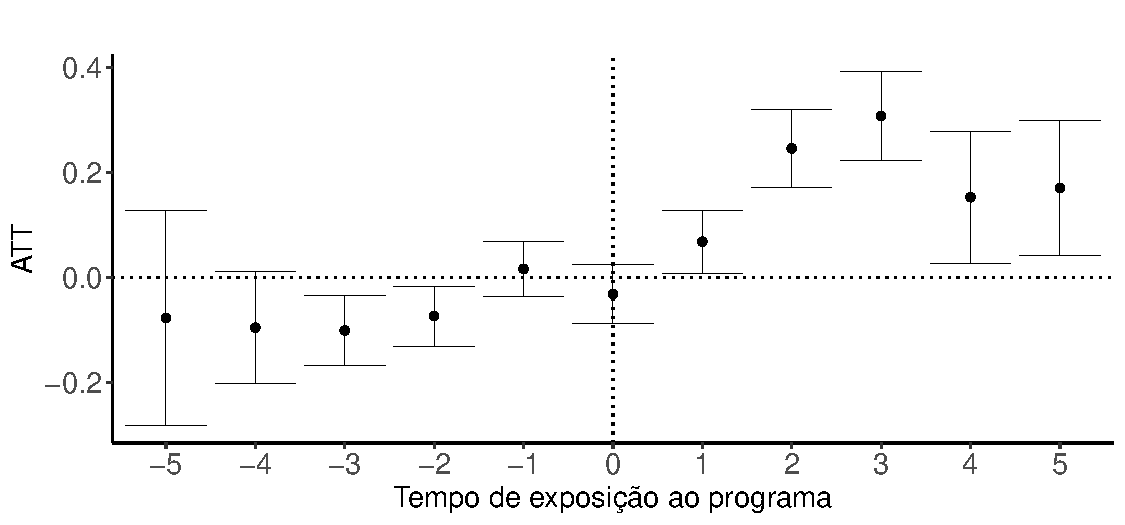
\includegraphics[width=1\linewidth]{Charts/did_agg_matematica.pdf}  
  \caption{Matemática}
  \label{fig:efeito_matematica}
\end{subfigure}
\begin{subfigure}{.5\textwidth}
  \centering
  % include second image
  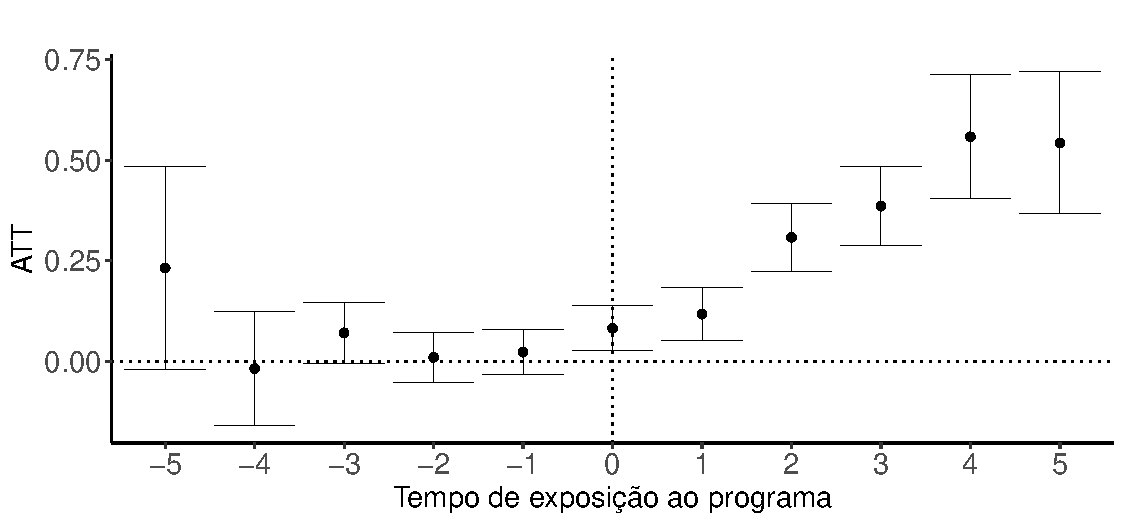
\includegraphics[width=1\linewidth]{Charts/did_agg_linguagem.pdf}  
  \caption{Linguagens}
  \label{fig:efeito_linguagem}
\end{subfigure}\newline

\begin{subfigure}{.5\textwidth}
  \centering
  % include third image
  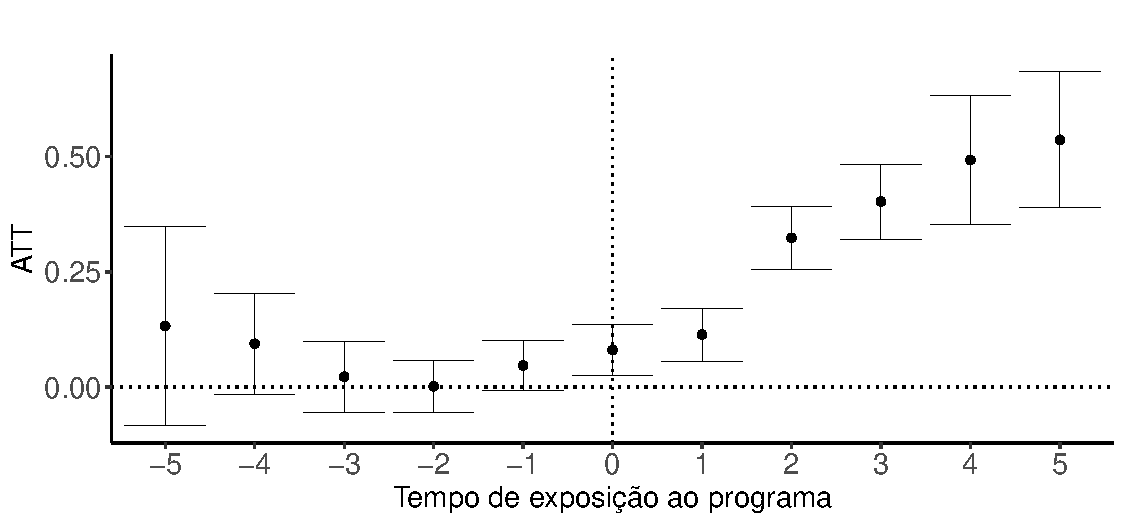
\includegraphics[width=1\linewidth]{Charts/did_agg_ciencias.pdf}  
  \caption{Ciências Naturais}
  \label{fig:efeito_ciencias}
\end{subfigure}
\begin{subfigure}{.5\textwidth}
  \centering
  % include fourth image
  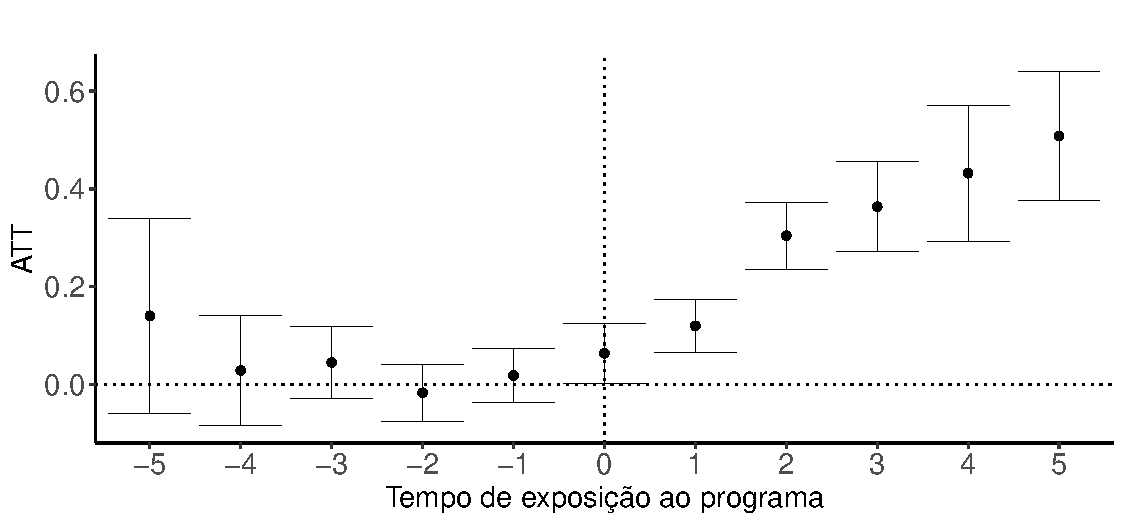
\includegraphics[width=1\linewidth]{Charts/did_agg_humanas.pdf}  
  \caption{Ciências Humanas}
  \label{fig:efeito_humanas}
\end{subfigure}
\begin{subfigure}{.5\textwidth}
  \centering
  % include first image
  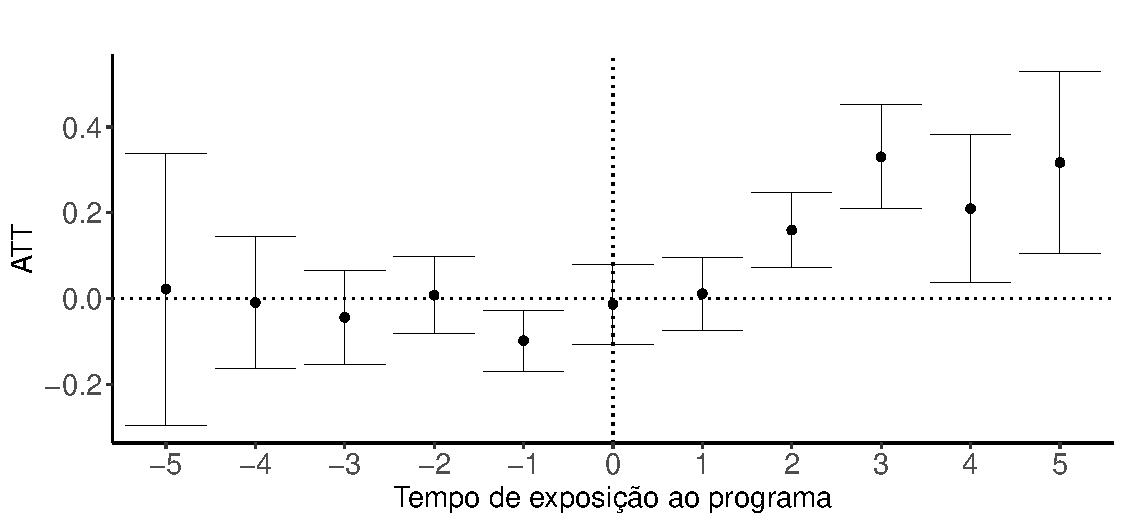
\includegraphics[width=1\linewidth]{Charts/did_agg_redacao.pdf}  
  \caption{Redação}
  \label{fig:efeito_redacao}
\end{subfigure}
\begin{subfigure}{.5\textwidth}
  \centering
  % include fourth image
  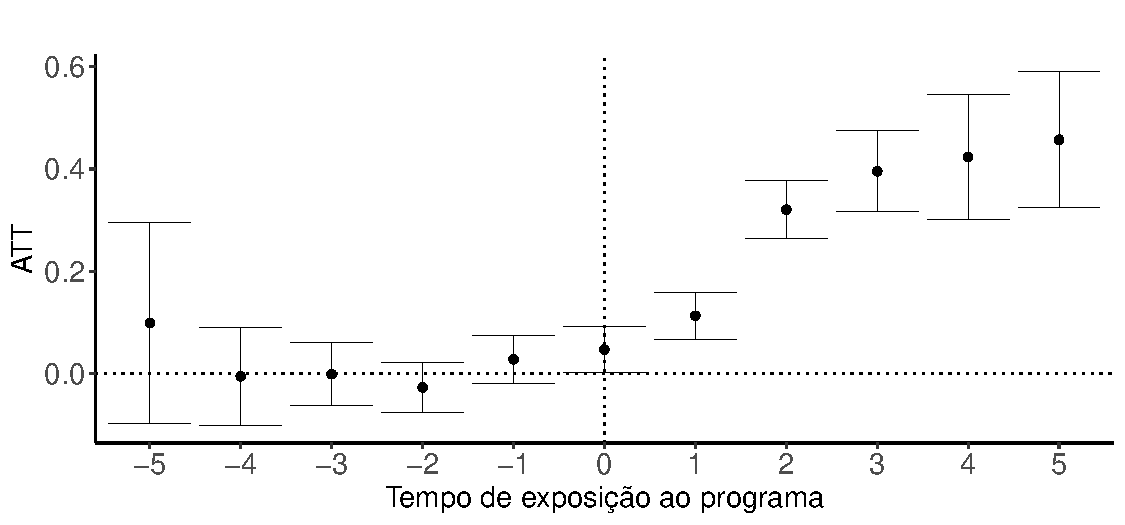
\includegraphics[width=1\linewidth]{Charts/did_agg_objetiva.pdf}  
  \caption{Geral em Objetivas}
  \label{fig:efeito_objetiva}
\end{subfigure}
\legend{Fontes: Elaboração própria, 2024}
\label{fig:efeito_agg_objetivas}
\end{figure}

\begin{figure}[b]
\caption{Efeito agregado sobre indicadores educacionais}
\begin{subfigure}{.5\textwidth}
  \centering
  % include first image
  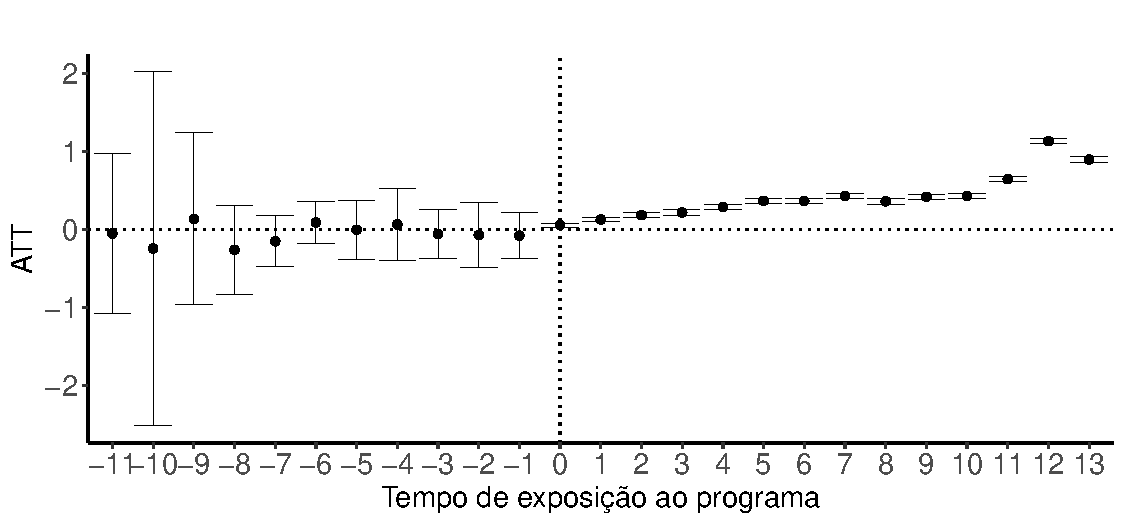
\includegraphics[width=1\linewidth]{Charts/did_agg_aprovacao.pdf}  
  \caption{Aprovação}
  \label{fig:efeito_aprovacao}
\end{subfigure}
\begin{subfigure}{.5\textwidth}
  \centering
  % include second image
  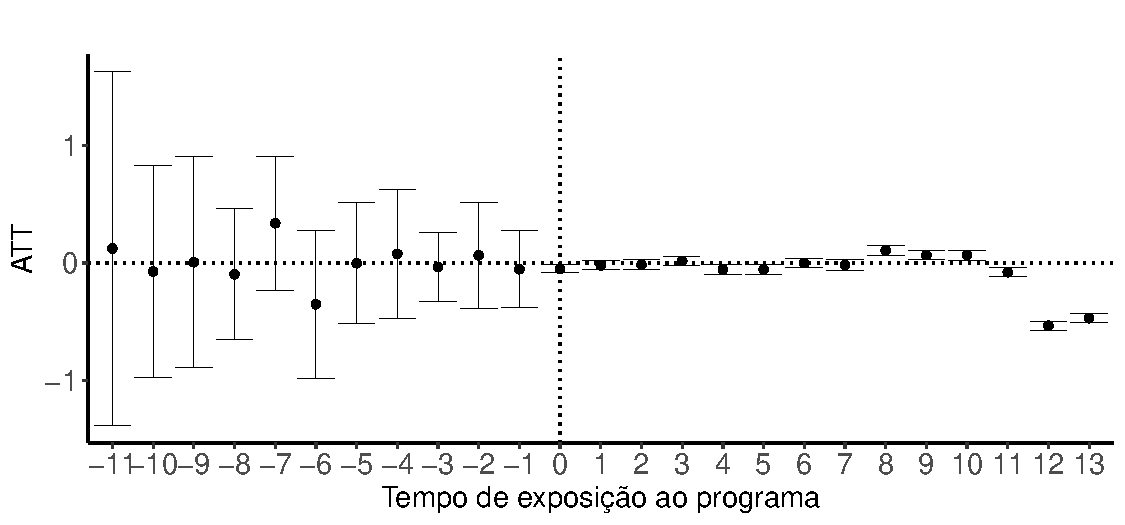
\includegraphics[width=1\linewidth]{Charts/did_agg_reprovacao.pdf}  
  \caption{Reprovação}
  \label{fig:efeito_reprovacao}
\end{subfigure}\newline

\begin{subfigure}{.5\textwidth}
  \centering
  % include third image
  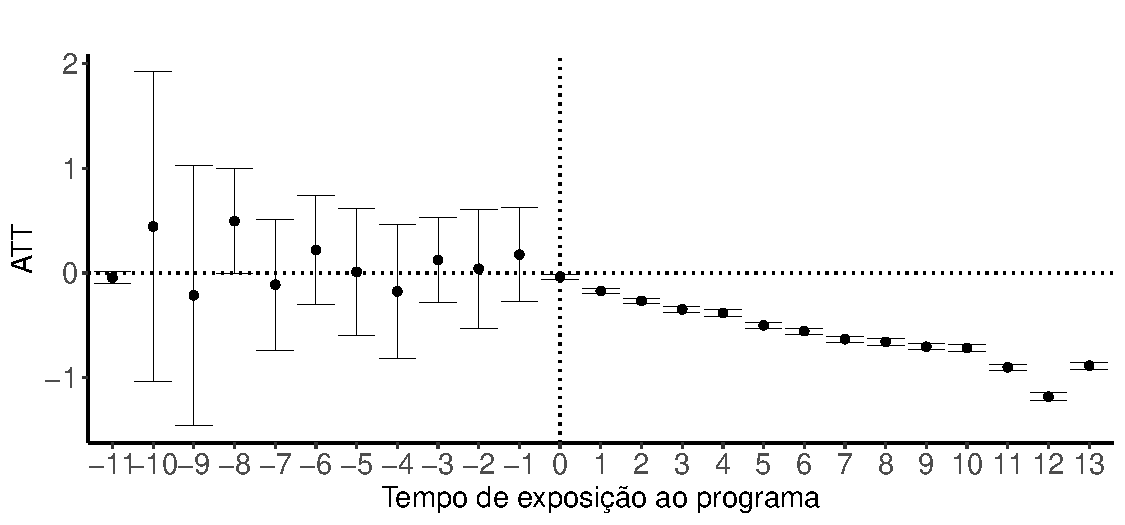
\includegraphics[width=1\linewidth]{Charts/did_agg_abandono.pdf}  
  \caption{Abandono}
  \label{fig:efeito_abandono}
\end{subfigure}
\begin{subfigure}{.5\textwidth}
  \centering
  % include fourth image
  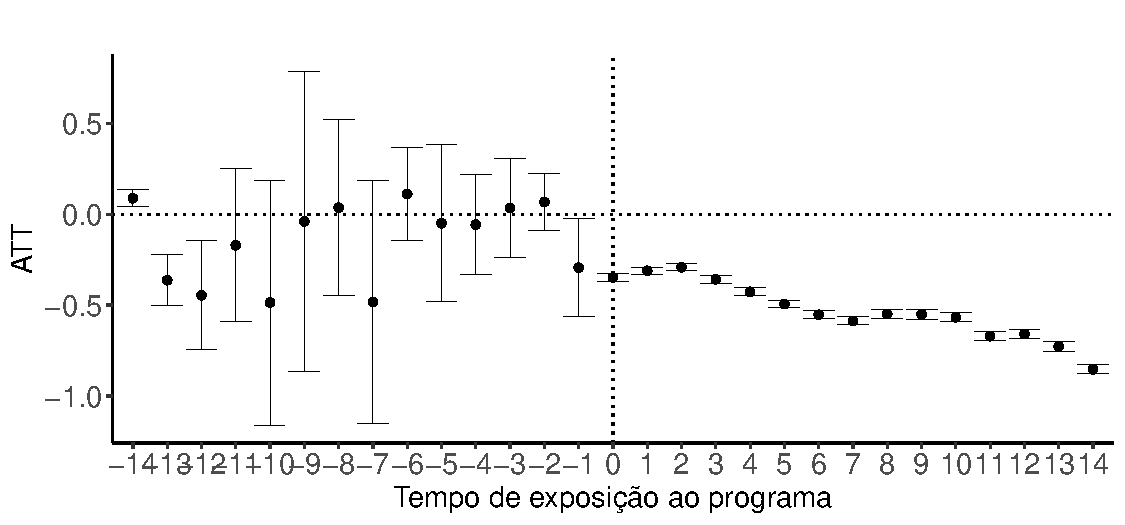
\includegraphics[width=1\linewidth]{Charts/did_agg_distorcao.pdf}  
  \caption{Distorção}
  \label{fig:efeito_distorcao}
\end{subfigure}

\legend{Fontes: Elaboração própria, 2024}
\label{fig:efeito_agg_indicadores}
\end{figure}